% Created 2022-10-02 Sun 11:33
% Intended LaTeX compiler: pdflatex
\documentclass[11pt]{article}
\usepackage[utf8]{inputenc}
\usepackage[T1]{fontenc}
\usepackage{graphicx}
\usepackage{longtable}
\usepackage{wrapfig}
\usepackage{rotating}
\usepackage[normalem]{ulem}
\usepackage{amsmath}
\usepackage{amssymb}
\usepackage{capt-of}
\usepackage{hyperref}
\AddToHook{cmd/section/before}{\clearpage}
\graphicspath{{../../books/}}
% TIPS
% \substack{a\\b} for multiple lines text





% pdfplots will load xolor automatically without option
\usepackage[dvipsnames]{xcolor}

\usepackage{forest}
% two-line text in node by [two \\ lines]
% \begin{forest} qtree, [..] \end{forest}
\forestset{
  qtree/.style={
    baseline,
    for tree={
      parent anchor=south,
      child anchor=north,
      align=center,
      inner sep=1pt,
    }}}
%\usepackage{flexisym}
% load order of mathtools and mathabx, otherwise conflict overbrace

\usepackage{mathtools}
%\usepackage{fourier}
\usepackage{pgfplots}
\usepackage{amsthm, mathabx,  amsmath, commath}
\usepackage{amsfonts}

\usepackage{empheq}
\usepackage{tikz}
\usetikzlibrary{arrows.meta}
\usepackage[most]{tcolorbox}

\newtheorem{theorem}{Theorem}[section]
\newtheorem{definition}{Definition}[section]
\newtheorem{corollary}{Corollary}[section]
\newtheorem{example}{Example}[section]
\newtheorem{lemma}{Lemma}[section]
\newtheorem{proposition}{Proposition}[section]

\newcommand{\bl}[1] {\boldsymbol{#1}}
\newcommand{\Wt}[1] {\stackrel{\sim}{\smash{#1}\rule{0pt}{1.1ex}}}
\newcommand{\wt}[1] {\widetilde{#1}}


%For boxed texts in align, use Aboxed{}
%otherwise use boxed{}

\DeclareMathSymbol{\widehatsym}{\mathord}{largesymbols}{"62}
\newcommand\lowerwidehatsym{%
  \text{\smash{\raisebox{-1.3ex}{%
    $\widehatsym$}}}}
\newcommand\fixwidehat[1]{%
  \mathchoice
    {\accentset{\displaystyle\lowerwidehatsym}{#1}}
    {\accentset{\textstyle\lowerwidehatsym}{#1}}
    {\accentset{\scriptstyle\lowerwidehatsym}{#1}}
    {\accentset{\scriptscriptstyle\lowerwidehatsym}{#1}}
}

\usepackage{graphicx}
    
% text on arrow for xRightarrow
\makeatletter
%\newcommand{\xRightarrow}[2][]{\ext@arrow 0359\Rightarrowfill@{#1}{#2}}
\makeatother


\def \bx {\boldsymbol{x}}
\def \ba {\boldsymbol{a}}
\def \bI {\boldsymbol{I}}
\def \bt {\boldsymbol{t}}
\def \bb {\boldsymbol{b}}
\def \bA {\boldsymbol{A}}
\def \bX {\boldsymbol{X}}
\def \bu {\boldsymbol{u}}
\def \bS {\boldsymbol{S}}
\def \bZ {\boldsymbol{Z}}
\def \bz {\boldsymbol{z}}
\def \by {\boldsymbol{y}}
\def \bw {\boldsymbol{w}}
\def \bT {\boldsymbol{T}}
\def \bS {\boldsymbol{S}}
\def \bm {\boldsymbol{m}}
\def \bW {\boldsymbol{W}}
\def \bY {\boldsymbol{Y}}
\def \bH {\boldsymbol{H}}
\def \blambda {\boldsymbol{\lambda}}
\def \bPhi {\boldsymbol{\Phi}}
\def \btheta {\boldsymbol{\theta}}
\def \bmu {\boldsymbol{\mu}}
\def \bphi {\boldsymbol{\phi}}
\def \bSigma {\boldsymbol{\Sigma}}
\def \lb {\left\{}
\def \rb {\right\}}
\def \caln {\mathcal{N}}
\def \dissum {\displaystyle\Sigma}
\def \dispro {\displaystyle\prod}
\def \E {\mathbb{E}}
\def \Q {\mathbb{Q}}
\def \V {\mathbb{V}}
\def \R {\mathbb{R}}
\def \calq {\mathcal{Q}}
\def \calg {\mathcal{G}}
\def \caln {\mathcal{N}}
\def \calr {\mathcal{R}}
\def \calm {\mathcal{M}}
\def \calc {\mathcal{C}}
\def \bcup {\bigcup}

\makeindex
\usepackage{minted}
\renewcommand*{\proofname}{Solution}
\let\OldTexttt\texttt
\renewcommand{\texttt}[1]{\OldTexttt{\color{MidnightBlue} #1}}
\author{wu}
\date{\today}
\title{Competitive programming}
\hypersetup{
 pdfauthor={wu},
 pdftitle={Competitive programming},
 pdfkeywords={},
 pdfsubject={},
 pdfcreator={Emacs 28.0.92 (Org mode 9.6)}, 
 pdflang={English}}
\begin{document}

\maketitle
\tableofcontents


\section{Dynamic Programming}
\label{sec:org4c535ef}
\subsection{General}
\label{sec:orgc2f70cc}
\begin{problem}[\href{https://leetcode.cn/problems/find-all-good-indices/}{LeetCode: Find All Good Indices}]
You are given a \emph{0-indexed} integer array nums of size \(n\) and a positive integer \(k\).

We call an index \(i\) in the range \(k\le i< n-k\) good if the following conditions are satisfied:
\begin{itemize}
\item The \(k\) elements that are just before the index \(i\) are in non-increasing order.
\item The \(k\) elements that are just after the index \(i\) are in non-decreasing order.
\end{itemize}

Return an array of all good indices sorted in increasing order.
\end{problem}

\begin{proof}
For \(j\), suppose the non-increasing elements before \(j\) (including \(j\)) is \(left_j\), the
non-decreasing elements after \(j\) (including \(j\)) is \(right_j\), then \(i\) is good iff
\(left_{i-1}\ge k\) and \(right_{i+1}\ge k\)
\end{proof}

\begin{problem}[\href{https://leetcode.cn/problems/get-kth-magic-number-lcci/}{LeetCode: Get Kth Magic Number}]
Design an algorithm to find the kth number such that the only prime factors are 3, 5, and 7.
Note that 3, 5, and 7 do not have to be factors, but it should not have any other prime factors.
For example, the first several multiples would be (in order) 1, 3, 5, 7, 9, 15, 21.
\end{problem}

\begin{proof}
We can use heap: for each element \(x\) took out, add \(3x,5x,7x\) into the heap. Also we need
to eliminate the duplicates

Define \(dp[i]\) is the \(i\)th number, so \(dp[1]=1\), and let \(p_3=p_5=p_7=1\) initially, then
for \(2 \le i\le k\)
\begin{equation*}
dp[i]=\min(dp[p_3]\cdot 3, dp[p_5]\cdot 5, dp[p_7]\cdot 7)
\end{equation*}
and increment the corresponding \(p_k\) where \(k\in\{3,5,7\}\)
\end{proof}

\begin{problem}[\href{https://leetcode.cn/problems/remove-boxes/}{LeetCode: Remove Boxes}]
You are given several boxes with different colors represented by different positive numbers.

You may experience several rounds to remove boxes until there is no box left. Each time you can
choose some continuous boxes with the same color (i.e., composed of \(k\) boxes, \(k\ge 1\)), remove
them and get \(k^2\) points.

\emph{Return the maximum points you can get.}
\end{problem}

\begin{proof}
Let \(dp(l,r,k)\) denote the maximum points we can get in boxes \([l,r]\) if we have extra \(k\)
boxes which is the same color with \(boxes[l]\) in the left side.

For example, if \texttt{boxes=[3,3,1,3,3]}, then \(dp(3,4,2)\) is the maximum we can get in \texttt{boxes[3,4]} if
we have extra 2 boxes the same color with \texttt{boxes[3]} in the left side

Since \((a+b)^2>a^2+b^2\) where \(a>0,b>0\), it's better to greedy to remove all contiguous boxes
of the same color, instead of split them. So we increase both \(l\) and \(k\) while
\texttt{boxes[l+1]==boxes[l]}

Now we have some options:
\begin{itemize}
\item remove all boxes which has the same color with boxes \(l\), total points we can get is
\(dp(l+1,r,0)+(k+1)^2\)
\item merge non-contiguous boxes of the same color together, by
\begin{itemize}
\item find the index \(j\) where \(l+1\le j\le r\) so that \texttt{boxes[j]==boxes[l]}
\item total points we can get is \(dp(j,r,k+1)+dp(l+1,j-1,0)\)
\end{itemize}
\end{itemize}

\begin{figure}[htbp]
\centering
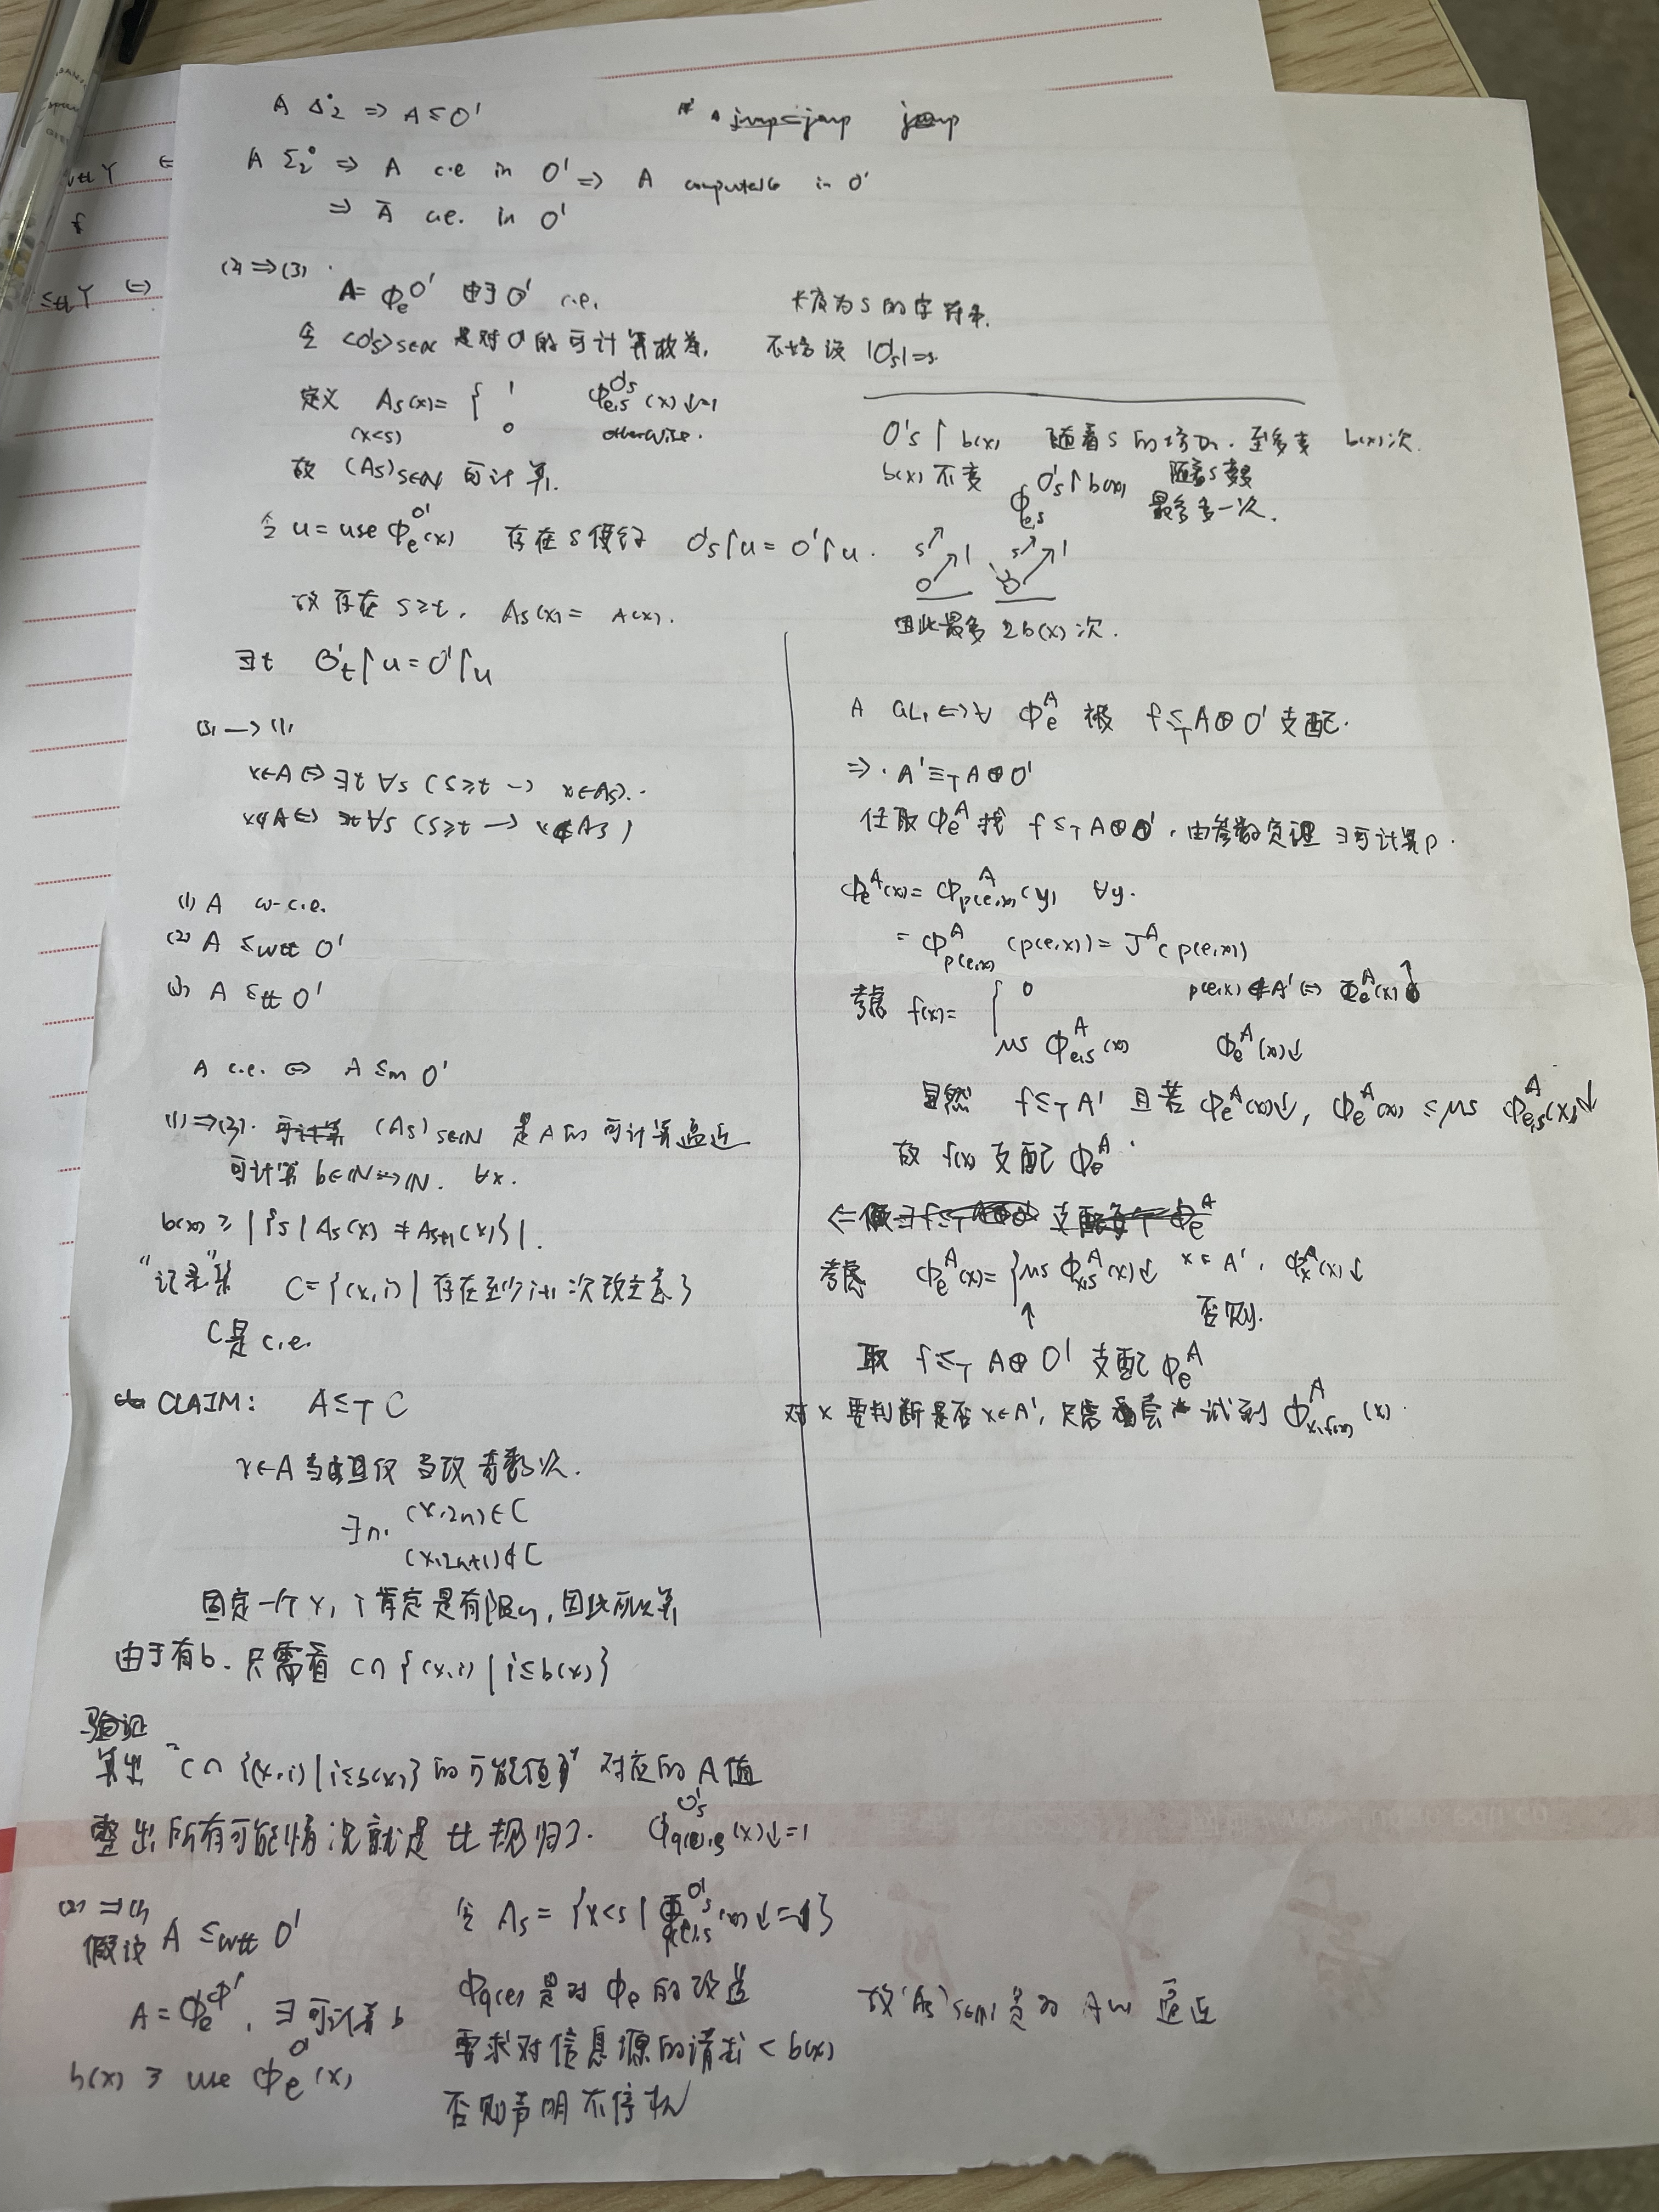
\includegraphics[width=.6\textwidth]{../images/cp/1.png}
\label{}
\end{figure}
\end{proof}



\subsection{Digit DP}
\label{sec:orgfe04150}
\begin{problem}[LeetCode 788: Rotated Digits]
An integer x is a \textbf{good} if after rotating each digit individually by 180 degrees, we get a valid
number that is different  from x. Each digit must be rotated - we cannot choose to leave it alone.

A number is valid if each digit remains a digit after rotation. For example:
\begin{itemize}
\item 0, 1, and 8 rotate to themselves,
\item 2 and 5 rotate to each other (in this case they are rotated in a different direction, in other
words, 2 or 5 gets mirrored)
\item 6 and 9 rotate to each other, and
\item the rest of the numbers do not rotate to any other number and become invalid.
\end{itemize}

Given an integer n, return the number of good integers in the range [1, n].
\end{problem}

\begin{proof}
Given \(n\).
Let \(f(pos,bound,diff)\) be the number of good numbers satisfying
\begin{enumerate}
\item Only consider \(pos\)th digit and \(pos\) starts from left, which means 0th digit is the
highest digit. And we assume the first \(pos-1\)
digits are fixed
\item If digits in \([0,pos-1]\) are first \(pos\) digits of \(n\), then \(bound\) is \texttt{true}
\item If digits in \([0,pos-1]\) has at least one 2/5/6/9, then \(diff\) is \texttt{true}
\end{enumerate}

Therefore the answer is \(f(0, true, false)\), and the transition formula is
\begin{equation*}
f(pos,bound,diff)=\sum f(pos+1,bound',diff')
\end{equation*}
\begin{itemize}
\item \(bound'\) is true iff \(bound\) is true and the digit we choose is the \(pos\)th digit
of \(n\)
\item \(diff'\) is true iff \(diff\) is true or we chose 2/5/6/9
\end{itemize}
\end{proof}
\section{Graph}
\label{sec:org57a33e6}
\subsection{Union find}
\label{sec:orgf58b309}
\begin{problem}[\href{https://leetcode.cn/problems/number-of-good-paths/}{LeetCode: Number of Good Paths}]
There is a tree (i.e. a connected, undirected graph with no cycles) consisting of \(n\) nodes
numbered from 0 to \(n-1\) and exactly \(n - 1\) edges.

You are given a 0-indexed integer array \texttt{vals} of length \(n\) where \texttt{vals[i]} denotes the value of the
\(i\)th node. You are also given a 2D integer array edges where \texttt{edges[i] = [ai,bi]} denotes that
there exists an undirected edge connecting nodes \(a_i\) and \(b_i\).

A good path is a simple path that satisfies the following conditions:
\begin{enumerate}
\item The starting node and the ending node have the same value.
\item All nodes between the starting node and the ending node have values less than or equal to the
starting node (i.e. the starting node's value should be the maximum value along the path).
\end{enumerate}

\emph{Return the number of distinct good paths.}

Note that a path and its reverse are counted as the same path. For example, \texttt{0 -> 1} is considered
to be the same as \texttt{1 -> 0}. A single node is also considered as a valid path.
\end{problem}

\begin{proof}
First, to solve the problem, we can enumerate the paths from the nodes with largest \texttt{vals}, and
then delete these nodes and continue; this requires \(O(n^2)\) time

If we reverse the direction, we are merging nodes with values from low to high, so what comes to
our mind? Union find.

For each node \(s\) and its neighbor \(t\):
\begin{enumerate}
\item if \texttt{vals[s]<vals[t]}, then pass
\item if \texttt{vals[s]=vals[find[t]]}, then add \texttt{size[find[s]]*size[find[t]]}
\item merge \texttt{s} and \texttt{t}
\end{enumerate}
\end{proof}

\section{General}
\label{sec:org6106e7a}
\subsection{Intervals}
\label{sec:orge624c25}
\begin{problem}[\href{https://leetcode.cn/problems/count-days-spent-together/}{LeetCode: Count Days Spent Together}]
Alice and Bob are traveling to Rome for separate business meetings.

You are given 4 strings \texttt{arriveAlice}, \texttt{leaveAlice}, \texttt{arriveBob}, and \texttt{leaveBob}. Alice will be in the
city from the dates \texttt{arriveAlice} to \texttt{leaveAlice} (inclusive), while Bob will be in the city from
the dates \texttt{arriveBob} to \texttt{leaveBob} (inclusive). Each will be a 5-character string in the format
``MM-DD'', corresponding to the month and day of the date.

Return the total number of days that Alice and Bob are in Rome together.

You can assume that all dates occur in the same calendar year, which is not a leap year. Note
that the number of days  per month can be represented as: [31, 28, 31, 30, 31, 30, 31, 31, 30, 31, 30, 31].
\end{problem}

\begin{proof}
First we can convert the string to \(i\)th day of the year, then Alice's interval is \([a,b]\),
Bob's interval is \([c,d]\), then we need to calculate the intersection of these intervals.

\([a,b]\cap[c,d]\neq\emptyset\) iff \(b\ge c\wedge d\ge a\).

\([a,b]\cap[c,d]=\min(b,d)-\max(a,c)+1\)
\end{proof}

\subsection{Bit operation}
\label{sec:org3cf19cd}
\begin{problem}[\href{https://leetcode.cn/problems/missing-two-lcci/}{Leetcode: Missing Two LCCI}]
You are given an array with all the numbers from 1 to N appearing exactly once, except for two
number that is missing. How can you find the missing number in \(O(N)\) time and \(O(1)\) space?

You can return the missing numbers in any order.

\begin{center}
\begin{tabular}{ll}
Input & Output\\
\hline
\texttt{[1]} & \texttt{[2,3]}\\
\texttt{[2,3]} & \texttt{[1,4]}\\
\end{tabular}
\end{center}


\texttt{nums.length <= 30000}
\end{problem}

\begin{proof}
Suppose the missing two numbers are \(x_1\) and \(x_2\), and if we add \(1,\dots,N\) to the end of the
array \(A\), then \(x=\bigoplus A=x_1\oplus x_2\).

By \texttt{x\&-x} we can get the lowest bit of \(x\), assume it's in \(l\)th bit. Then we can
assume \(x_1\)'s \(l\)th bit is 0, and \(x_2\)'s \(l\)th bit is 1, and we can partition \(A\) into
\(A_1\) and \(A_2\) by whether the elements' \(l\)th bit is 1, then \(\bigoplus A_1=x_1\) and \(\bigoplus A_2=x_2\)
\end{proof}

\begin{problem}[\href{https://leetcode.cn/problems/find-a-value-of-a-mysterious-function-closest-to-target/}{LeetCode: Find a Value of a Mysterious Function Closest to Target}]
​
\begin{minted}[]{c++}
func(arr, l, r) {
  if (r < l) {
    return -10000000000;
  }
  ans = arr[l];
  for (i = l + 1; i <= r; i++) {
    ans = ans & arr[i];
  }
  return ans;
}
\end{minted}
Winston was given the above mysterious function \texttt{func}. He has an integer array \texttt{arr} and an integer
\texttt{target} and he wants to find the values \texttt{l} and \texttt{r} that make the value \texttt{|func(arr, l, r) - target|}
minimum possible.

Return the minimum possible value of \texttt{|func(arr, l, r) - target|}.

Notice that func should be called with the values l and r where \texttt{0 <= l, r < arr.length}.

Constraints:
\begin{itemize}
\item \texttt{1 <= arr.length <= 10\textasciicircum{}5}
\item \texttt{1 <= arr[i] <= 10\textasciicircum{}6}
\item \texttt{0 <= target <= 10\textasciicircum{}7}
\end{itemize}
\end{problem}

\begin{proof}
If we fix \(r\)
\begin{itemize}
\item \(f\) is a non-decreasing function
\item there is at most 20 different values for \(f(arr,l,r)\) as \(arr[r]\le 10^6<2^{20}\), since from
right to left, 0 won't be transformed into 1
\end{itemize}
\end{proof}

\begin{problem}[\href{https://leetcode.cn/problems/smallest-subarrays-with-maximum-bitwise-or/}{LeetCode: Smallest Subarrays With Maximum Bitwise OR}]
You are given a \emph{0-indexed} array nums of length \(n\), consisting of non-negative integers. For
each index \(i\) from 0 to \(n-1\), you must determine the size of the minimum sized non-empty
subarray of nums starting at \(i\) (inclusive) that has the maximum possible bitwise OR.

Return an integer array answer of size \(n\) where answer[i] is the length of the minimum sized subarray
starting at \(i\) with maximum bitwise OR.

A subarray is a contiguous non-empty sequence of elements within an array.
\end{problem}

\begin{proof}
Induction and we build a new array \(A=\{a_i:a_i=nums[i]\}\). In the \(i\)th round, for
each \(j<i\), check whether \(a_j|a_i>a_j\). If so, \(a_j|a_i\) is the new possible maximum
for \(a_j\) and the possible \(answer[j]\ge i-j+1\).

If \(a_j|a_i=a_j\), then \(a_i\subseteq a_j\) in the sense of bits and for
each \(k<j\), \(a_k|a_i=a_k|a_j\). So we don't need to consider \(k<j\)
\end{proof}
\subsection{Hard to say}
\label{sec:org41234af}
\begin{problem}[\href{https://leetcode.cn/problems/minimum-money-required-before-transactions/}{LeetCode: Minimum Money Required Before Transactions}]
You are given a 0-indexed 2D integer array transactions, where \texttt{transactions[i] = [costi, cashbacki]}.

The array describes transactions, where each transaction must be completed exactly once in some
order. At any given moment, you have a certain amount of money. In order to complete transaction
\(i\), \texttt{money >= cost\_i} must hold true. After performing a transaction, money becomes \texttt{money-cost\_i+cashback\_i}.

Return the minimum amount of money required before any transaction so that all of the
transactions can be completed regardless of the order of the transactions.
\end{problem}

\begin{proof}
The worst case is, we put money-losing transaction first and then put the transaction with
highest cost after it (erase the transaction before if necessary, and assume its index is \(i\))

Suppose \(total\) is the total lose, then if the transaction is money-losing, then the money we need is
\begin{equation*}
total-(cost[i]-cashback[i])+cost[i] = total+cashback[i]
\end{equation*}
Otherwise
\begin{equation*}
total+cost[i]
\end{equation*}
\end{proof}


\begin{problem}[\href{https://leetcode.cn/problems/sparse-similarity-lcci/}{LeetCode: Sparse Similarity}]
The similarity of two documents (each with distinct words) is defined to be the size of the
intersection divided by the size of the union. For example, if the documents consist of
integers, the similarity of \{1, 5, 3\} and \{1, 7, 2, 3\} is 0.4, because the intersection has size
2 and the union has size 5. We have a long list of documents (with distinct values and each with
an associated ID) where the similarity is believed to be ``sparse''. That is, any two arbitrarily
selected documents are very likely to have similarity 0. Design an algorithm that returns a list
of pairs of document IDs and the associated similarity.

Input is a 2D array docs, where docs[i] is the document with id i. Return an array of strings,
where each string represents a pair of documents with similarity greater than 0. The string
should be formatted as  \{id1\},\{id2\}: \{similarity\}, where id1 is the smaller id in the two
documents, and similarity is the similarity rounded to four decimal places. You can return the
array in any order.

return in any order.
\end{problem}

\begin{proof}
Assume we have \(D\) documents and each document has at most \(W\) words

Brute force: given two documents \(A, B\), answer
is \((\abs{A}+\abs{B}-\abs{A\cup B})/\abs{A\cup B}\), \(O(D^2W)\)

We use inverted index to optimize \(D^2\). We can build a hash table with key the elements of
documents and the value the index of the document.

Then to find the document with similarity > 0 with \(A\), we only need to check the hash value
for each element of \(A\)
\end{proof}
\end{document}
